\documentclass[conference]{IEEEtran}
\IEEEoverridecommandlockouts
% The preceding line is only needed to identify funding in the first footnote. If that is unneeded, please comment it out.
\usepackage{cite}
\usepackage{amsmath,amssymb,amsfonts}
\usepackage{algorithmic}
\usepackage{graphicx}
\usepackage{textcomp}
\usepackage{xcolor}
\usepackage{xurl}
\usepackage[utf8]{inputenc}
\def\BibTeX{{\rm B\kern-.05em{\sc i\kern-.025em b}\kern-.08em
    T\kern-.1667em\lower.7ex\hbox{E}\kern-.125emX}}
    
\newcommand{\bibRef}[1]
{\textsuperscript{\cite{#1}}}

 
\begin{document}

\title{
Touffu\\
{\footnotesize
Projet annuel (2022) - ESGI 3e année - Architecture Logicielle}
}

\author{
\IEEEauthorblockN{Nathan LETOURNEAU}
\IEEEauthorblockA{
\textit{Étudiant en Architecture Logicielle}\\
\textit{École Supérieure de Génie Informatique}\\
@Nathan-dev-dot\\
nathan.letourneau@net-c.com}
\and
\IEEEauthorblockN{Théo OMNES}
\IEEEauthorblockA{
\textit{Étudiant en Architecture Logicielle}\\
\textit{École Supérieure de Génie Informatique}\\
@NightTheo\\
omnes.theo@gmail.com}
\and
\IEEEauthorblockN{Sarah SCHLEGEL}
\IEEEauthorblockA{
\textit{Étudiante en Architecture Logicielle}\\
\textit{École Supérieure de Génie Informatique}\\
@SarahSch19\\
sschlegel@protonmail.ch}
}

\maketitle

\begin{abstract}
Le projet annuel de la filière Architecture Logicielle de l'ESGI a pour but de rassembler en un seul projet la plupart des compétences acquises au cours de l'année. En 2022, il s'articule autour des éléments suivants : réalisation d'un front-end en AngularJS, d'une application lourde en Java, d'une API en NodeJS, d'une base de données noSQL, d'une base de données relationnelle, et de la création d'un langage de scraping. Axé sur le thème de l'aide à la personne, il propose de combiner les éléments précédents afin de concevoir un service numérique complet.
\end{abstract}

\section{Introduction}

\textit{Touffu} est une application d'aide à la personne, centrée sur les soins et promenades d'animaux de compagnie pour les personnes dépendantes\bibRef{Soins aux animaux}. Le service a pour but de mettre en relation les personnes dépendantes, nécessitant de l'aide, avec des volontaires déclarés qui peuvent s'occuper des animaux domestiques\bibRef{Animaux domestiques}.\\

Au niveau technique, le service se divise en sept modules majeurs :
\begin{enumerate}
	\item Une application client en AngularJS, destinée aux utilisateurs principaux du service : elle permettra aux utilisateurs de s'inscrire et de trouver ou de proposer leurs services en fonction de leur catégorie ;
	\item Une application d'administration en AngularJS, destinée aux gérants de l'application, afin de gérer les comptes des utilisateurs, la base de données, les catégories principales de l'application, etc. ;
	\item Une API en NodeJS pour faire la jonction entre les deux applications front-end et la base de données ;
	\item Une base de données en noSQL, accessible à partir de l'API ;
	\item Une application lourde de gestion du projet Touffu en Java destinée aux développeurs de Touffu. Cette application doit notamment inclure une messagerie interne et une gestion de plugins.
	\item Une base de données relationnelle pour gérer les données associées au pilotage du projet, qui ne sera associée qu'à l'application Java.
	\item Un langage de scraping en ligne de commande permettant de récupérer des informations sur les prestations procurées (soins et promenades des animaux de compagnie pour les personnes dépendantes) à partir de différentes sources Web, pour les traiter et les enregistrer dans des fichiers.
\end{enumerate}
Ces modules sont représentés de manière graphique dans la figure \ref{fig:architecture}.

\begin{figure}[h]
    \centering
    
\includegraphics[width=\columnwidth]{Ressources/Images/Architecture.png}
    \caption{Architecture globale}
    \label{fig:architecture}
\end{figure}

\subsection{Descriptif du projet}

\begin{figure}[h]
	\centering
	
\includegraphics[width=0.4\columnwidth]{Ressources/Icons/v1_all.png}
	\caption{Logo Global}
	\label{fig:logotouffuall}
\end{figure}

\subsubsection{Touffu client ("Touffu")}\hfil

\begin{figure}[h]
	\centering
	
\includegraphics[width=0.4\columnwidth]{Ressources/Icons/v1_2@3x.png}
	\caption{Logo Touffu}
	\label{fig:logotouffu}
\end{figure}

Du côté front-end, en s'inscrivant sur Touffu, les utilisateurs définissent s'ils souhaitent être aidés (bénéficiaires ou personnes tierces demandant en leur nom) ou apporter de l'aide (prestataires). L'application leur permet ensuite de définir leurs besoins (promenade, brossage, préparation de nourriture, changement de litière, accompagnement chez le vétérinaire) ou leurs disponibilités (types d'animaux, activités, possibilité d'effectuer des prestations récurrentes ou ponctuelles).\\

Les bénéficiaires qui ont besoin d'aide peuvent définir si elles ont besoin d'une aide récurrente, auquel cas elles peuvent définir une récurrence quotidienne, hebdomadaire ou mensuelle par exemple, ou d'une intervention ponctuelle. Ils peuvent définir si cette demande concerne plusieurs animaux ou un seul, et à combien de temps ils estiment cette prestation. Dans le cadre d'une intervention chez le vétérinaire, ils définissent également s'ils peuvent fournir un moyen de transport ou payer les frais de transport et comment ils couvrent les frais du vétérinaire.

Le système montre ensuite à chacun des partis une liste de personnes qui correspondent à leurs besoins et leurs disponibilités. Un système de messagerie interne leur permet d'échanger au préalable s'ils souhaitent dialoguer. Un calendrier propre à chaque utilisateur rappelle ensuite l'évènement à l'utilisateur.\\

Le prestataire (ou aidant) peut de son côté travailler pour plusieurs bénéficiaires à la condition que ses activités chez différentes personnes ne se chevauchent pas. Il peut également exercer plusieurs activités (qui peuvent concerner des animaux différents) chez un seul bénéficiaire sur une même plage horaire.

Un système d'évaluation permet de noter la prestation d'un prestataire par le bénéficiaire, et inversement le comportement du bénéficiaire envers le prestataire. Cette évaluation est prise en compte dans la mise en avant des prestataires et des bénéficiaires dans les recherches. Elle est également mise en évidence dans les statistiques individuelles de chaque utilisateur, qui affichent donc en plus de sa note ses performances individuelles.\\

La plateforme Touffu permet de gérer en ligne les paiements des prestataires (via Stripe ou système similaire), ce qui permet également de générer les factures des prestataires. Les prestataires et les bénéficiaires peuvent se mettre d'accord sur la fréquence des facturations et des paiements (paiements à la prestation, hebdomadaires ou mensuels). En fonction du mode de paiement défini, le système affichera un rappel pour le bénéficiaire de la prestation et enverra une notification (mail) qui l'amènera au système de paiement.

Si le bénéficiaire est en retard sur ses paiements, des sanctions progressives seront appliquées (suspension des prestations en cours, blocage de nouvelles annonces, verrouillage du compte).
\\

\subsubsection{Front admin ("TouffAdmin")}\hfill\\

\begin{figure}[h]
	\centering
	
\includegraphics[width=0.4\columnwidth]{Ressources/Icons/v1_3@3x.png}
	\caption{Logo TouffAdmin}
	\label{fig:logotouffadmin}
\end{figure}

Le front d'administration servira au service de Touffu pour la gestion de l'application. Cela comprend notamment la gestion des comptes utilisateur, la gestion des offres et demandes (suppression d'arnaques, gestion et envois des factures), de vérifier les messages qui ont été signalés par les utilisateurs comme inappropriés.

Ce backend permet également de gérer les comptes administrateurs (ajouter ou supprimer des administrateurs ou des modérateurs, définir leurs droits individuels ou de groupe.\\

Le front client est également géré à partir du backend. Cela inclut de gérer l'apparence du front client (images sur les sliders, texte de présentation, titres, etc.) et les données dans les formulaires (contenu des listes des services disponibles).

Des statistiques sont générées régulièrement (tâche automatisée) pour évaluer les tendances dans les activités des prestataires et les demandes des bénéficiaires, et pouvoir afficher les tarifs moyens pour une prestation donnée.\\

Touffu prélève une commission sur le paiement en ligne, tant du côté du prestataire que du côté du bénéficiaire, afin de subvenir à ses propres besoins. Le pourcentage de cette marge est défini dans l'administration de Touffu.\\

\subsubsection{Gestion de projet ("Touffu-Management")}\hfil\\

\begin{figure}[h]
	\centering
	
\includegraphics[width=0.4\columnwidth]{Ressources/Icons/v1_1@3x.png}
	\caption{Logo Touffu Management}
	\label{fig:logotouffu-management}
\end{figure}

L'application de management est destinée aux développeurs de Touffu, afin qu'ils puissent préparer les différentes étapes du projet, ainsi que les ressources humaines associées. Le management se fait via une interface de type Trello, avec une gestion de tableaux (cf. figure \ref{fig:touffumanagementhomedesign}), colonnes et de cartes, également disponible en ligne de commande. Les utilisateurs peuvent ajouter, supprimer ou modifier des tableaux, cartes ou colonnes, et déplacer les cartes entre les colonnes.

Pour l'affectation des tâches, les utilisateurs peuvent s'affecter une tâche, ou l'affecter à un autre utilisateur présent sur le tableau.

Un transfert de droits sur un tableau peut avoir lieu si le propriétaire du tableau souhaite passer la main à un autre utilisateur. C'est le propriétaire d'un tableau (à l'origine son créateur donc) qui peut ajouter des membres à un tableau et gérer le tableau (suppression notamment).

Un gestionnaire de plugins intégré permet d'ajouter des plugins afin de rajouter des fonctionnalités aux tableaux. Par exemple, un plugin pourrait permettre d'ajouter des images à une carte, ou bien d'envoyer des notifications par email lors de la mise à jour d'une carte, ou encore d'ajouter des commentaires sur une carte.

Une messagerie interne permet aux utilisateurs de communiquer sur l'avancée du projet. Cette messagerie est propre à chaque utilisateur, et lui permet d'échanger avec un autre des utilisateurs de l'application.

Enfin, un système d'export permet d'exporter un tableau au format PDF.\\

\subsubsection{Scraper ("Touffu Scrap")}\hfill\\

Le langage compilé de Touffu permettra dans la mesure de raisonnable de scrapper toutes les données du site client Touffu et d'autres sites similaires (récupérer des types de balises, les valeurs qu'elles contiennent...).

\subsection{Fonctionnalités optionnelles}
\begin{itemize}
	\item Application mobile (Swift, "TouffApp") avec géolocalisation pour les promenades des animaux
	\item Système d'abonnement payant à Touffu pour les prestataires leur donnant des accès à des fonctionnalités plus pointues (liste non-exhaustive : statistiques détaillées, export des calendriers)
\end{itemize}


\section{Fonctionnalités}

\subsection{Interface utilisateur / Touffu}

\subsubsection{Gestion des utilisateurs}\hfil\\

\textbf{Inscription}\\
- Affichage de la page d'inscription\\
- L'utilisateur renseigne son email (doit être unique dans l'instance de la base de données), son téléphone, un mot de passe et son nom complet (nom, prénom), et sélectionne s'il souhaite demander de l'aide ou en proposer\\
- L'application vérifie le format du numéro de téléphone (préfixe de région + type de numéro par région), l'unicité de l'email et la complexité du mot de passe (longueur supérieure à 8 caractères, au moins une majuscule, une minuscule, un chiffre et un caractère spécial)\\

Cas 1 : L'email est déjà utilisé\\
- Affichage d'un message d'erreur\\

Cas 2 : L'email n'est pas utilisé\\
- Affichage des champs d'inscription détaillés en fonction de la catégorie sélectionnée par l'utilisateur\\

Cas 2.1 : L'utilisateur propose son aide\\
- L'utilisateur sélectionne les animaux dont il souhaite s'occuper, ses types de prestations (récurrentes ou ponctuelles), ses disponibilités (jours et heures dans la semaine) et son rayon d'action géographique\\

Cas 2.2 : L'utilisateur a besoin d'aide\\
- L'utilisateur définit son emplacement géographique et liste son ou ses animaux\\
- Pour chaque animal, il définit les prestations nécessaires (promenade, brossage, préparation de nourriture, changement de litière, accompagnement chez le vétérinaire) et leur fréquence (quotidienne, hebdomadaire, mensuelle, ponctuelle)\\
- Dans le cas d'une prestation récurrente, l'utilisateur définit s'il le souhaite une date de début et de fin de la récurrence\\

Cas 2.1 et 2.2 - terminaison :\\
- Le système enregistre les données et crée le compte de l'utilisateur\\
- Le système transfère l'utilisateur à la page de connexion en affichant un message de succès\\

\textbf{Connexion}\\
- Affichage d'une fenêtre de connexion\\
- L'utilisateur entre ses identifiants de connexion (email et mot de passe)\\
- L'application vérifie la combinaison des identifiants\\

Cas 1 : Combinaison invalide\\
- La fenêtre affiche un message d'erreur\\
Cas 2 : Combinaison valide\\
- L'utilisateur est redirigé vers la page d'accueil de l'espace utilisateurs\\

\textbf{Gestion du profil}\\
- Affichage de la page de profil de l'utilisateur\\

Cas 1 : L'utilisateur est un prestataire\\
- L'utilisateur modifie les animaux dont il souhaite s'occuper, ses types de prestations (récurrentes ou ponctuelles), ou ses disponibilités (jours et heures dans la semaine)\\

Cas 2 : L'utilisateur est un bénéficiaire\\
- Pour chaque animal, l'utilisateur définit les prestations nécessaires (promenade, brossage, préparation de nourriture, changement de litière, accompagnement chez le vétérinaire) et leur fréquence (quotidienne, hebdomadaire, mensuelle, ponctuelle)\\

Cas 1 et 2 - terminaison :\\
- Le système enregistre les données et affiche un message de confirmation\\

\textbf{Gestion du compte}\\
- Affichage de la page des préférences de l'utilisateur
- L'utilisateur modifie des données liées à son compte (email de contact, numéro de téléphone, mot de passe)\\
- Dans le cas du mot de passe, le système valide la complexité du mot de passe (longueur supérieure à 8 caractères, au moins une majuscule, une minuscule, un chiffre et un caractère spécial)\\
- Dans le cas de l'email, le système vérifie qu'il n'est pas déjà attribué à un autre utilisateur\\
- L'utilisateur entre son mot de passe courant pour valider les changements\\
- Le système enregistre les données, génère un log de modification, et affiche un message de confirmation\\
- Le système envoie un email à l'utilisateur pour l'informer des modifications apportées à son compte. Cet email contient un lien afin d'annuler les changements et d'avertir le support si ce n'est pas lui qui a effectué la modification\\

\textbf{Suppression de compte}\\
- Affichage de la fenêtre des paramètres de l'utilisateur\\
- L'utilisateur sélectionne \textit{Supprimer le compte} dans la danger zone\\
- Le système supprime toutes les données de l'utilisateur, et le retire de toutes les cartes où il était désigné en tant que personne assignée à la tâche\\


\subsubsection{Gestion des offres}\hfil\\

Le système de prestations est basé sur une acceptation mutuelle de l'offre par le prestataire et par le bénéficiaire.\\

\textbf{Acceptation d'une offre}\hfil\\
Pour le prestataire :\\
- Affichage de la liste des besoins des bénéficiaires\\
- Le prestataire sélectionne une offre et propose son aide\\
- L'application met à jour l'offre avec un statut \textit{En attente de confirmation} et envoie un email au bénéficiaire pour l'informer du changement\\

Pour le bénéficiaire\\
- Affichage de la page de l'offre en attente de confirmation, avec les informations des différents prestataires ayant proposé leur aide\\
- Le bénéficiaire accepte ou refuse l'aide du prestataire\\
- Le système enregistre le choix du bénéficiaire\\

Terminaison 1 : Le bénéficiaire accepte la proposition\\
- Le système envoie un email au prestataire pour l'informer de l'acceptation\\
- Le système met à jour les calendriers du prestataire et du bénéficiaire\\

Terminaison 2 : Le bénéficiaire refuse la proposition\\
- Le système envoie un email au prestataire pour l'informer du refus\\

\textbf{Suspension d'une offre}\hfil\\
- Affichage de la page des offres du bénéficiaire\\
- Le bénéficiaire sélectionne l'offre qu'il souhaite suspendre\\
- Le système affiche les détails de l'offre\\
- Le bénéficiaire suspend l'offre\\
- Le système met à jour l'offre en base de données\\

\textbf{Suppression d'une offre}\hfil\\
- Affichage de la page des offres du bénéficiaire\\
- Le bénéficiaire sélectionne l'offre qu'il souhaite suspendre\\
- Le système affiche les détails de l'offre\\
- Le bénéficiaire suspend l'offre\\
- Le système supprime l'offre en base de données\\


\subsubsection{Gestion des prestations}\hfil\\

\textbf{Annulation d'une prestation}\hfil\\
- Affichage de la page d'une prestation en attente\\
- Le prestataire renseigne un motif d'annulation\\

Cas 1 : Prestation ponctuelle\\
- Le système envoie un email au bénéficiaire l'informant de l'annulation\\

Cas 2 : Prestation récurrente\\
- Le prestataire spécifie s'il annule une seule prestation ou s'il annule toutes les prestations à venir\\

Cas 2.1 : Annulation d'une seule prestation\\
- Le système envoie un email au bénéficiaire l'informant de l'annulation\\

Cas 2.2 : Annulation de toutes les prestations (résiliation d'un accord de prestations récurrentes)\\
- Voir la section \textit{Résiliation d'un accord}\\

\textbf{Résiliation d'un accord}\hfil\\
Par "accord", on définit une prestation récurrente acceptée par le bénéficiaire et le prestataire. Étant donné qu'un accord engage le prestataire pour une prestation récurrente, une date de préavis de résiliation est à prévoir. Cette durée est définie au moment de l'accord, dans l'\textit{Acceptation de l'offre}.\\

- Affichage de la page d'une offre\\
- Le prestataire sélectionne \textit{Résilier l'accord} et la date de résiliation de ses services au bénéficiaire\\
- Le système demande une confirmation et avertit des conséquences en cas de préavis non-respecté\\
- Le prestataire confirme\\
- Le système enregistre l'annulation du service et, en fonction de la durée du préavis, applique une amende sur la rémunération du prestataire\\

\textbf{Évaluation d'une prestation}\hfil\\
Prérequis :\\
- À la fin d'une prestation, le système envoie un email au bénéficiaire et au prestataire contenant un lien vers un formulaire d'évaluation\\

- Affichage de la page contenant le formulaire d'évaluation\\
- L'utilisateur et le bénéficiaire saisissent leur évaluation sur la prestation de la journée (accueil, disponibilité, ponctualité, réalisation de la demande)\\
- Le système enregistre l'évaluation en base de données et recalcule les scores de chaque utilisateur\\
- Lorsque le prestataire et le bénéficiaire ont chacun évalué, le système rend les résultats de l'évaluation disponible aux deux\\

\textbf{Rémunération d'une prestation}\\
La rémunération des prestations est conditionnée par le type de prestation. Une prestation ponctuelle est rémunérée au moment de la prestation. Pour cela, le bénéficiaire de la prestation dispose d'un délai d'une semaine pour payer la prestation. Une prestation récurrente est rémunérée mensuellement, et un malus est appliqué en cas de non exécution de la prestation.\\

- Affichage de la page d'une prestation récurrente en cours ou d'une prestation ponctuelle exécutée\\
- L'utilisateur sélectionne \textit{Rémunérer la prestation}\\
- Le système redirige l'utilisateur vers la page de paiement pré-remplie avec les informations du paiement de la prestation\\
- Le bénéficiaire entre ses données de paiement\\
- Le système vérifie et valide le paiement avec le système tiers de paiement en ligne\\

\textbf{Téléchargement d'une facture}\hfil\\
- Affichage d'une prestation qui a été rémunérée\\
- L'utilisateur choisit de télécharger la facture\\
- Le système génère et télécharge la facture sur le poste de l'utilisateur\\

\subsection{Interface administrateur / TouffAdmin}\hfil\\

\subsubsection{Gestion des utilisateurs}\hfil\\

\textbf{Connexion}\\
- Affichage d'une page de connexion\\
- L'utilisateur entre ses identifiants de connexion (email et mot de passe)\\
- L'application vérifie la combinaison des identifiants

Cas 1 : Combinaison invalide\\
- La fenêtre affiche un message d'erreur\\
Cas 2 : Combinaison valide\\
- L'utilisateur est redirigé vers la page d'accueil de l'espace utilisateurs\\

\textbf{Modification de mot de passe}\\
- Affichage d'une page de

\subsection{Pilotage du projet / Touffu Management}

La gestion du projet Touffu se fait au travers d'une application Java avec une interface graphique similaire à celle de Trello, comme le montre la figure \ref{fig:touffumanagementhomedesign}. La vue principale d'un projet se divise en colonnes, dans lesquelles des cartes affichent les différentes tâches.\\
Les fonctionnalités suivantes sont décrites sous la forme graphique, mais une version de l'application est également disponible en ligne de commande, auquel cas les traitements sont les mêmes, à l'exception de la gestion des fenêtres d'affichage.

\begin{figure}[h]
	\centering
	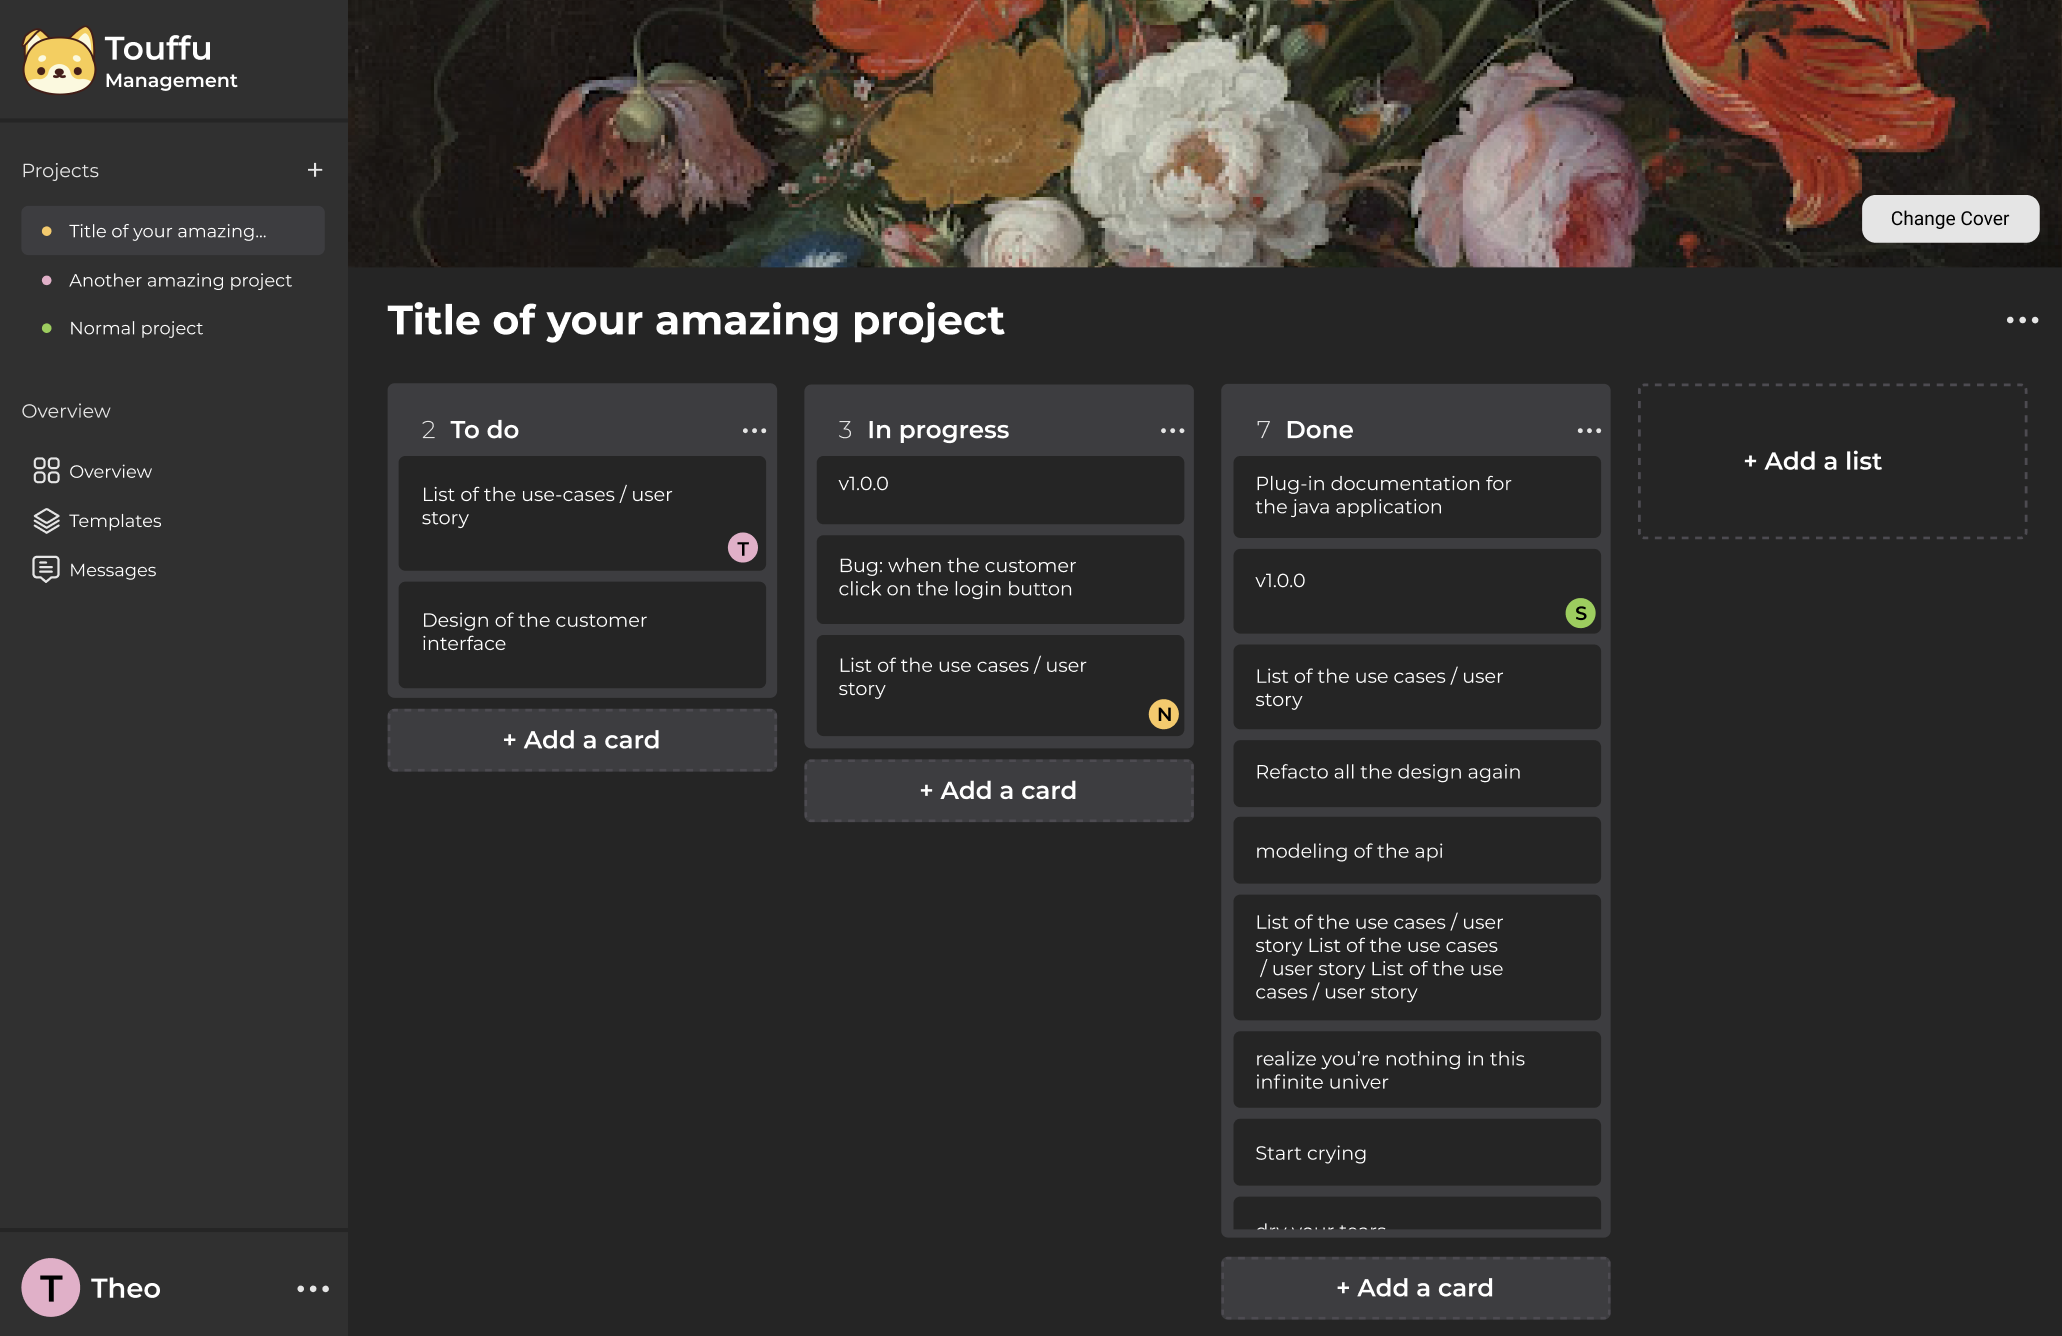
\includegraphics[width=\columnwidth]{Ressources/Images/Touffu-management-home}
	\caption{Management app - home design}
	\label{fig:touffumanagementhomedesign}
\end{figure}

\subsubsection{Gestion des utilisateurs}\hfil\\

\textbf{Inscription}\\
- Affichage d'une fenêtre d'inscription\\
- L'utilisateur renseigne son email (doit être unique dans l'instance de la base de données), un mot de passe et son nom complet (nom, prénom)\\
- L'application vérifie l'unicité de l'email et insère les données en base de données\\
- L'application envoie un email de confirmation d'inscription à l'utilisateur\\
- L'utilisateur est redirigé vers la fenêtre de connexion\\

\textbf{Connexion}\\
- Affichage d'une fenêtre de connexion\\
- L'utilisateur entre ses identifiants de connexion (email et mot de passe)\\
- L'application vérifie la combinaison des identifiants\\
- En cas d'erreur, la fenêtre affiche un message d'erreur\\
- En cas de succès, l'utilisateur est redirigé vers la page d'accueil\\

\textbf{Suppression de compte}\\
- Affichage de la fenêtre des paramètres de l'utilisateur\\
- L'utilisateur sélectionne \textit{Supprimer le compte} dans la danger zone\\
- Le système supprime toutes les données de l'utilisateur, et le retire de toutes les cartes où il était désigné en tant que personne assignée à la tâche\\

\begin{figure}[h]
	\centering
	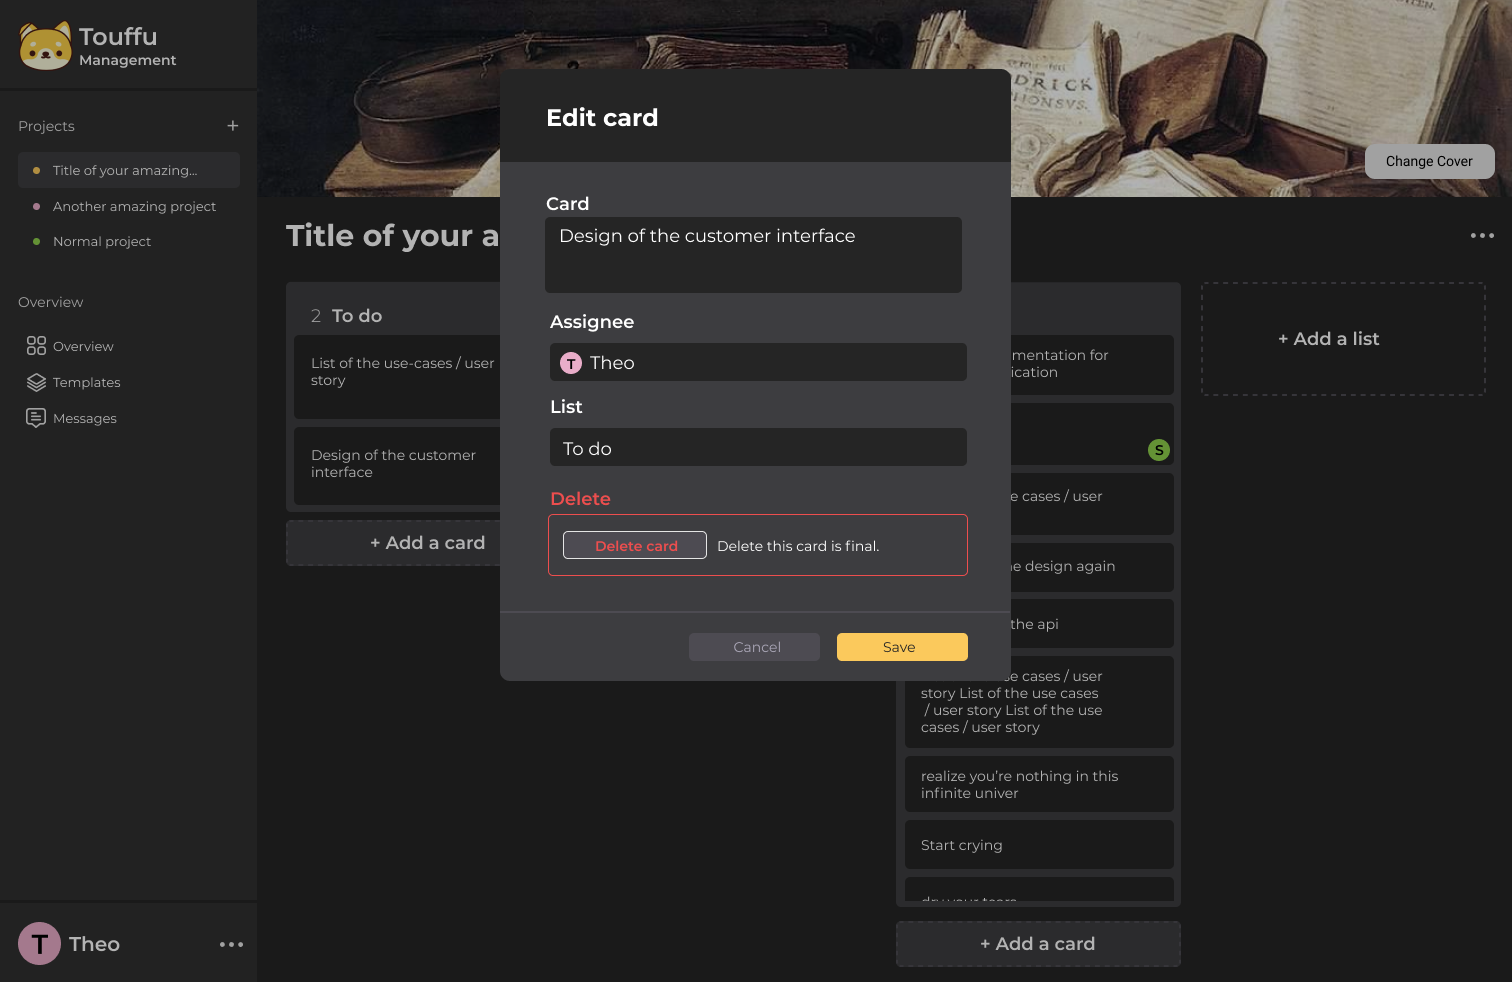
\includegraphics[width=\columnwidth]{Ressources/Images/Touffu-management-edit-card}
	\caption{Management app - éditer une carte}
	\label{fig:touffumanagementeditcard}
\end{figure}


\subsubsection{Gestion des projets et des tâches}\hfil\\

\textbf{Création d'un projet}\\
- Affichage d'une fenêtre pour créer un nouveau projet\\
- L'utilisateur entre le nom du projet, \textbf{(la deadline et ?)} choisit une image de fond\\
- Le système insère le projet en base de données\\
- Le système enregistre l'image dans les données de l'application \textbf{(...-> Serveur, bdd, local...?)}\\

\textbf{Modification d'un projet}\\
- Affichage de la fenêtre de modification du projet\\
- L'utilisateur modifie le champ du projet qu'il souhaite modifier (nom, couleur, etc.).\\
- Le système enregistre les changements\\

\textbf{Ajout d'un utilisateur à un projet}\\
- Affichage de la fenêtre de modification du projet\\
- Dans la section \textit{Membres}, l'utilisateur clique sur le bouton \textit{Ajouter un membre}\\
- L'utilisateur entre l'email de la personne\\
- L'application envoie un email pour informer l'utilisateur qu'il a été ajouté dans le projet\\

\textbf{Suppression d'un projet}\\
- Affichage de la fenêtre de modification du projet\\
- L'utilisateur clique sur le champ \textit{Supprimer le projet} dans la danger zone\\
- Le système supprime le projet et toutes les cartes, listes et tâches associées en base de données\\

\textbf{Ajout d'une liste}\\
- Affichage d'une fenêtre de création de liste\\
- L'utilisateur entre le nom de la nouvelle liste\\
- L'application ajoute la liste en base de données et l'affiche sur le tableau du projet\\

\textbf{Modification d'une liste}\\
- Affichage de la fenêtre de modification de la liste\\
- L'utilisateur modifie le champ de la liste qu'il souhaite modifier (nom).\\
- Le système enregistre les changements\\

\textbf{Suppression d'une liste}\\
- Affichage de la fenêtre de modification de la liste\\
- L'utilisateur clique sur le champ \textit{Supprimer la liste} dans la danger zone\\
- Le système supprime la liste ainsi que les tâches qu'elle contenait\\

\textbf{Ajout d'une tâche}\\
- Affichage d'une fenêtre d'ajout d'une carte\\
- L'utilisateur entre le nom de la carte, ainsi qu'un utilisateur assigné à cette tâche (facultatif)\\
- L'application ajoute la tâche en base de données et affiche la carte dans la liste associée\\

\textbf{Modification d'une tâche}\\
- Affichage de la fenêtre de modification de la tâche\\
- L'utilisateur modifie le champ de la tâche qu'il souhaite modifier (nom, utilisateur associé, liste).\\
- Le système enregistre les changements\\

\textbf{Suppression d'une tâche}\\
- Affichage de la fenêtre de modification de la tâche\\
- L'utilisateur clique sur le champ \textit{Supprimer la carte} dans la danger zone\\
- Le système supprime la carte\\

\textbf{Export PDF}\\
- To do\\

\subsubsection{Gestion des plugins}

\subsubsection{Messagerie interne}\hfill\\

La messagerie d'un utilisateur lui permet d'échanger avec les différents membres de son équipe. Les messages se font entre deux utilisateurs donnés.\\

\textbf{Affichage d'une conversation}\\
- L'utilisateur clique sur l'icône d'un autre utilisateur dans une carte\\
- Le système ouvre la messagerie sur la conversation avec cet utilisateur\\
OU\\
- L'utilisateur ouvre la messagerie\\
- Le système ouvre la page par défaut de la messagerie\\
- L'utilisateur sélectionne une conversation déjà entamée dans la liste de ses conversations\\

\textbf{Lancement d'une conversation}\\
- Affichage de la fenêtre par défaut de la messagerie\\
- L'utilisateur clique sur le bouton \textit{+ (Nouvelle conversation)}
- Le système affiche un champ de recherche\\
- L'utilisateur entre le nom, le prénom ou l'email de l'utilisateur avec qui il souhaite initier une conversation\\
- Le système recherche dans la liste des utilisateurs de l'application une correspondance\\
- Si aucune correspondance n'est trouvée, la fenêtre affiche un message d'erreur\\
- Si une ou plusieurs correspondances sont trouvées, l'utilisateur sélectionne le bon utilisateur\\
- L'application ouvre une fenêtre d'envois de messages\\

\textbf{Envoi d'un message}\\
Prérequis : Affichage d'une conversation\\
- L'utilisateur envoie un message par le champ d'envoi\\
- Le système enregistre le message\\

\subsection{Récupération de données (Scraping)}
…

\section{Environnement de développement}

\subsection{Décisions logicielles}
…

\subsection{Estimation des coûts}
…

\section{Spécifications}
…

\section{Architecture logicielle}

\subsection{Architecture globale}

…

\subsection{Organisation des répertoires}

Le projet est développé et versionné sous Git, dans une organisation appelée touffu-esgi\bibRef{touffu-esgi}, et administré par les développeurs. L'organisation comporte six "repos" majeurs, qui sont les dossiers des modules de l'application. Ces repos sont indépendants les uns des autres en termes de code propre, mais interdépendants en ce qui concerne la donnée, tel que le montre la figure \ref{fig:architecture}.\\

\subsubsection*{Touffu\bibRef{Touffu} }

Le répertoire Touffu contient le front-end principal, soit l'application client en AngularJS.\\

\subsubsection*{TouffAdmin\bibRef{TouffAdmin} }

TouffAdmin est le repository du backend administratif de l'application Touffu, lui aussi en AngularJS\\

\subsubsection*{TouffApi\bibRef{TouffApi} }

Le répertoire TouffApi contient les éléments de l'API en NodeJS.\\

\subsubsection*{Touffu-Management\bibRef{Touffu-Management} }

Ce répertoire est dédié à l'application lourde en Java.\\

\subsubsection*{Touffu-noSQL\bibRef{Touffu-noSQL} }

Le répertoire Touffu-noSQL contient toutes les données relatives à la base de données NoSQL.\\

\subsubsection*{Touffu-Scrap\bibRef{Touffu-Scrap} }

Touffu-Scrap est le répertoire destiné au langage de scraping développé par touffu-esgi afin de récupérer des données sur Internet au sujet des services à la personne.\\

\subsection{Architecture des modules}

\subsubsection*{Touffu}
\hfil\\
…\\

\subsubsection*{TouffAdmin}
\hfil\\
…\\

\subsubsection*{TouffApi}
\hfil\\
…\\

\subsubsection*{Touffu-Management}
\hfil\\
…\\

\subsubsection*{Touffu-noSQL}
\hfil\\
…\\

\subsubsection*{Touffu-Scrap}
\hfil\\
…\\

\section{Implémentation}

\begin{enumerate}
	\item \textbf{Inscription bénéficiaire :} En tant que bénéficiaire je souhaite m'inscrire avec les informations suivantes :
	\\Nom, prénom, adresse, email, téléphone, mot de passe
	\item \textbf{Inscription prestataire :} En tant que prestataire je souhaite m'inscrire avec les informations suivantes :
	\\Nom, prénom, adresse, email, téléphone, mot de passe, rayon d'action, prestations acceptées
	\item \textbf{Connexion bénéficiaire :} En tant que bénéficiaire je souhaite me connecter à mon compte
	\item \textbf{Connexion prestataire :} En tant que prestataire je souhaite me connecter à mon compte
	\item \textbf{Ajouter un animal de compagnie :} En tant que bénéficiaire je souhaite ajouter un animal de compagnie
	\\Nom de l'animal, type d'animal
	\item \textbf{Connexion bénéficiaire :} En tant que bénéficiaire je souhaite éditer un animal de compagnie
	\\Nom de l'animal, type d'animal
	\item \textbf{Déposer une demande d'aide :} En tant que bénéficiaire, je souhaite déposer une demande d'aide pour un animal
	\\Animal concerné, type de prestation, détails autres si nécessaire, durée de la prestation, fréquence de la prestation, horaires, rémunération
	\item \textbf{Consulter les offres des bénéficiaires :} En tant que prestataire, je souhaite consulter les offres disponibles des bénéficiaires en fonction de mes paramètres de recherche :
	\\Distance au domicile, type d'animal, type et fréquence de prestation
	\item \textbf{Proposer son aide :} En tant que prestataire, je souhaite proposer mon aide sur l'offre d'un bénéficiaire
	\item \textbf{Envoyer un message sur une offre :} En tant que bénéficiaire ou prestataire je peux envoyer un message sur une offre
	\item \textbf{Accepter une proposition d'aide :} En tant que bénéficiaire je souhaite accepter la proposition de l'un des prestataires
	\item \textbf{Noter une prestation :} En tant que bénéficiaire, je souhaite noter la prestation effectuée
	\item \textbf{Noter un bénéficiaire :} En tant que prestataire je souhaite noter le bénéficiaire chez qui j'ai effectué une prestation
	\item \textbf{Consulter son calendrier :} En tant que prestataire ou bénéficiaire, je souhaite afficher le calendrier de mes prestations ou offres courantes
	\item \textbf{Payer une prestation ponctuelle :} En tant que bénéficiaire, je souhaite payer un prestataire pour une prestation unique
	\item \textbf{Payer une prestation récurrente :} En tant que bénéficiaire, je souhaite payer le bénéficiaire en fin de mois pour un ensemble de prestations récurrentes
	\item \textbf{Annuler une prestation récurrente :} En tant que prestataire, je souhaite annuler une prestation récurrente que j'effectue chez un bénéficiaire
	\item \textbf{Annuler une occurrence d'une prestation récurrente :} En tant que prestataire, je souhaite annuler une occurrence d'une prestation récurrente que j'effectue chez un bénéficiaire
	\item \textbf{Annuler une offre :} En tant que bénéficiaire, je souhaite annuler une offre que j'ai déposée
	\\Si l'offre est récurrente et est déjà en cours d'exécution par un prestataire, je dois déposer un préavis de 7 jours pour ne pas être facturé
	\item \textbf{Suspendre une offre récurrente :} En tant que bénéficiaire, je souhaite suspendre une occurrence d'une offre que je propose
\end{enumerate}





\begin{thebibliography}{00}

\bibitem{Soins aux animaux}
\url{https://www.servicesalapersonne.gouv.fr/beneficier-des-sap/quelles-sont-activites-de-services-la-personne/soins-et-promenades-d-animaux-de-compagnie-pour-personnes-dependantes}

\bibitem{Animaux domestiques}
\url{https://www.legifrance.gouv.fr/jorf/id/JORFTEXT000000789087
}

\bibitem{touffu-esgi}
\url{https://github.com/touffu-esgi}

\bibitem{Touffu}
\url{https://github.com/touffu-esgi/Touffu}

\bibitem{TouffAdmin}
\url{https://github.com/touffu-esgi/TouffAdmin}

\bibitem{Touffu-Management}
\url{https://github.com/touffu-esgi/Touffu-Management}

\bibitem{TouffApi}
\url{https://github.com/touffu-esgi/TouffApi}

\bibitem{Touffu-Scrap}
\url{https://github.com/touffu-esgi/Touffu-Scrap}

\bibitem{Touffu-noSQL}
\url{https://github.com/touffu-esgi/Touffu-noSQL}

\end{thebibliography}


\end{document}
